% Drawing 154/02-23 -- folder 154, batch 02, archive page 35 (PDF page 36).
% Transcription: figures, colonne de droite : au milieu, une droite $L$ (vert clair et vert foncé) passant par un sommet $s$ où se coupent $D_1$ et $D_2$ (orange), traversée d'autres pseudo-droites, une petite flèche le long de $L$ et, dans une accolade, « la rive » ; au bas, un disque au bord vert (foncé à gauche, clair à droite), traversé de pseudo-droites orange dont deux, $D_1$ et $D_2$, vont du haut au bas du bord, où leurs extrémités sont marquées ; des régions au bord et au centre sont coloriées en jaune
% Kind: line L through a vertex of D1 and D2; disk crossed by pseudo-lines. Method 2 (schematic redraw from the facsimile). Status: ok.
% Notes: Upper figure: L light green, overdrawn in dark green on both sides of s; D_1 (the long thin stroke) and D_2 cross at s on L, a third stroke passes through s as well; three strokes cross L on the left and five on the right; the small arrow, the letter L and the words « la rive » in their brace-like stroke. Lower figure: Rim dark green on the left, light green on the right, with a short dark arc at the upper right and two short blue-grey arcs between the ends of D_1 and D_2 at the top and at the bottom; a pencil arrow outside the rim at the upper left. Ten orange strands followed from rim to rim (three from top to bottom, among them D_1 and D_2; six across; one down the right side), ends put on the rim; eight coloured regions, the four at the rim bounded by the rim and their strands, the four inner ones placed as read. The order of the crossings near the centre is a reading. Redrawn 2026-11-12 (issue 128). 2026-11-14, Claude Opus 5.5, second pass (issue 147): the upper figure redrawn stroke by stroke from the 400 dpi colour crop, every stroke through points measured on the colour mask of its ink along rows and columns of a unit grid: the long thin D_1 (it was a straight line up to 3 units off at its upper end), five more orange strokes (up to 2.5 units off; one of them, at the right, had its ends swapped), the dark green doubling of L on both sides of s (up to 1.8 units off) and the light green L. Overlay: every orange, light green and dark green stroke of both figures lies on the colour mask of its ink (mean distance under 0.3 unit, none more than 1 unit off over more than a tenth of its length); the strands of the lower disk were already on their ink. The order of the crossings near the centre of the disk is read from the ink, as drawn. Not compiled (no TeX in the session). Not checked by a reader.
% Coordinates: 1 unit = 1 mm = 1/100 of the crop width (bbox in page fractions: [0.51, 0.265, 0.78, 0.53]).
% Redrawn by Claude (claude-fable-5-2), issue #128, 2026-11-12; not checked by a human; not compiled (no TeX in the session).
% Redrawn stroke by stroke by Claude (claude-opus-5-5) 2026-11-14 (issue #147, second pass): overlaid on the 400 dpi colour facsimile on a unit grid; not compiled (no TeX in the session). Not checked by a human. Status: ok.
% Rights: reproduces part of the work -- behind RENDER_TRANSCRIPTS, never published by itself.
\documentclass[tikz,border=3pt]{standalone}
\usepackage{amsmath,amssymb}
\usetikzlibrary{patterns,arrows.meta}
\tikzset{Or/.style={orange!90!black}, Ye/.style={yellow!80!orange}, Lg/.style={green!60!black!70}, Dg/.style={green!45!black}, Bl/.style={blue!70!black}, pencil/.style={black!45}, struck/.style={black!35}, mpt/.style={circle,draw,inner sep=1.3pt}, pt/.style={circle,fill,inner sep=0.9pt}, opt/.style={circle,draw,fill=white,inner sep=1.1pt}}
\begin{document}
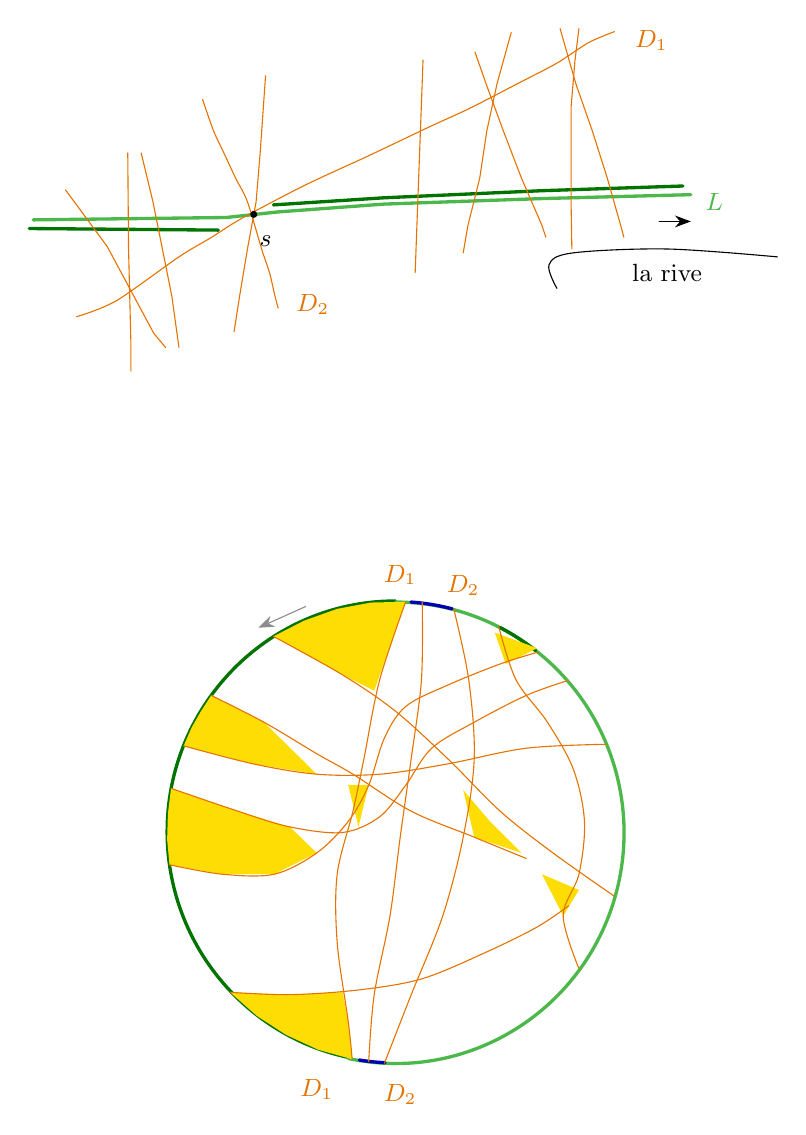
\begin{tikzpicture}[x=1mm,y=1mm,line cap=round,line join=round,font=\scriptsize]
\draw[Lg,very thick] (5.5,-26.3) -- (30,-26) -- (36.5,-25.3) -- (50,-24.3) -- (70,-23.6) -- (89,-23.1);
\draw[Dg,very thick] (5,-27.4) -- (29,-27.6);
\draw[Dg,very thick] (36,-24.4) -- (50,-23.5) -- (70,-22.6) -- (88,-22);
\draw[Or] plot[smooth, tension=0.5] coordinates {(11,-38.6) (16,-36.6) (24,-31) (28,-28.6) (32,-26.1) (40,-21.9) (48,-18.2) (56,-14.4) (61,-12.1) (67,-9) (72,-6.4) (76,-3.8) (79.3,-2.4)};
\draw[Or] plot[smooth, tension=0.5] coordinates {(27,-11) (28.4,-15) (29.8,-18) (31.2,-21) (32.7,-24) (34.5,-30) (35.5,-33) (36.2,-36) (36.6,-37.5)};
\draw[Or] (35,-8) -- (34.3,-18) -- (33.8,-24) -- (32.7,-30) -- (31.7,-36) -- (31,-40.5);
\draw[Or] (9.6,-22.5) -- (14.9,-29.7) -- (20.8,-40.7) -- (22.3,-42.5);
\draw[Or] (19.2,-17.8) -- (20.7,-24) -- (21.9,-30) -- (23.1,-36) -- (24,-42.5);
\draw[Or] (17.5,-17.8) -- (17.6,-30) -- (17.9,-42) -- (17.9,-45.5);
\draw[Or] (55,-6) -- (54,-33);
\draw[Or] (61.6,-5) -- (63,-9) -- (65.2,-15) -- (67.5,-21) -- (70.1,-27) -- (70.6,-28.5);
\draw[Or] (66.2,-2.5) -- (64.4,-9) -- (63.1,-15) -- (62.2,-21) -- (60.7,-27) -- (60.1,-30.5);
\draw[Or] (72.4,-2) -- (74.4,-9) -- (76.5,-15) -- (78.4,-21) -- (80.1,-27) -- (80.5,-28.5);
\draw[Or] (74.8,-2) -- (74.3,-6) -- (73.8,-12) -- (73.8,-24) -- (73.9,-30);
\node[pt] at (33.5,-25.6) {};
\draw[-{Stealth[length=2mm]}] (85,-26.5) -- (89,-26.5);
\node[inner sep=1pt,Lg] at (92,-24) {\small $L$};
\node[inner sep=1pt,Or] at (84,-3.5) {\small $D_1$};
\node[inner sep=1pt,Or] at (41,-37) {\small $D_2$};
\node[inner sep=1pt] at (35,-29) {\small $s$};
\draw plot[smooth, tension=0.55] coordinates {(72,-35) (71,-32) (74,-30.5) (86,-30) (100,-31)};
\node[inner sep=1pt] at (86,-33) {\small la rive};
\draw[Dg,very thick] (51.5,-74.7) arc[start angle=90, end angle=258, x radius=29, y radius=29.3];
\draw[Lg,very thick] (45.5,-132.8) arc[start angle=258, end angle=450, x radius=29, y radius=29.3];
\draw[Dg,very thick] (69.3,-81) arc[start angle=52, end angle=62.6, x radius=29, y radius=29.3];
\draw[Bl,very thick] (58.7,-75.7) arc[start angle=75.5, end angle=86, x radius=29, y radius=29.3];
\draw[Bl,very thick] (46.9,-133) arc[start angle=260.9, end angle=267.4, x radius=29, y radius=29.3];
\fill[pattern=north east lines,Ye] (52.8,-74.8) -- (48.4,-74.9) -- (44.1,-75.7) -- (39.9,-77.2) -- (36,-79.2) -- (44.8,-84.1) -- (48.8,-86.1) -- cycle;
\fill[pattern=north east lines,Ye] (28.1,-86.7) -- (26.8,-88.7) -- (25.6,-90.8) -- (24.6,-93.1) -- (33.5,-95.4) -- (41.5,-96.7) -- (34.8,-90.1) -- cycle;
\fill[pattern=north east lines,Ye] (23,-98.5) -- (22.6,-101.7) -- (22.5,-105) -- (22.8,-108.2) -- (29.5,-109.4) -- (36.1,-109.4) -- (41.5,-106.7) -- (38.1,-103.4) -- (31.5,-101.4) -- cycle;
\fill[pattern=north east lines,Ye] (30.5,-124.4) -- (33.9,-127.4) -- (37.6,-129.8) -- (41.7,-131.7) -- (46,-132.9) -- (45.5,-128.1) -- (44.8,-124.4) -- (38.1,-124.7) -- cycle;
\fill[pattern=north east lines,Ye] (45.5,-98.1) -- (48.1,-98.1) -- (46.8,-103.4) -- cycle;
\fill[pattern=north east lines,Ye] (60.1,-98.7) -- (63.5,-102.7) -- (67.5,-106.7) -- (61.5,-104.7) -- cycle;
\fill[pattern=north east lines,Ye] (70.1,-109.4) -- (74.8,-111.4) -- (72.8,-114.7) -- cycle;
\fill[pattern=north east lines,Ye] (64.1,-78.7) -- (69.5,-80.7) -- (65.5,-82.7) -- cycle;
\draw[Or] plot[smooth, tension=0.55] coordinates {(52.8,-74.8) (49.5,-84.7) (47.5,-94.7) (46.1,-101.4) (44.1,-109.4) (44.1,-118.1) (45.5,-128.1) (46,-132.9)};
\draw[Or] plot[smooth, tension=0.55] coordinates {(54.9,-74.9) (54.8,-84.7) (53.5,-94.7) (52.1,-104.7) (50.8,-114.7) (48.8,-124.7) (48.1,-133.2)};
\draw[Or] plot[smooth, tension=0.55] coordinates {(58.9,-75.7) (60.8,-84.7) (61.5,-94.7) (60.1,-104.7) (57.5,-114.7) (53.5,-124.7) (50.1,-133.4)};
\draw[Or] plot[smooth, tension=0.55] coordinates {(36,-79.2) (44.8,-84.1) (51.5,-88.7) (58.1,-94.7) (64.8,-101.4) (71.5,-106.7) (79.3,-112.2)};
\draw[Or] plot[smooth, tension=0.55] coordinates {(28.1,-86.7) (34.8,-90.1) (41.5,-94.1) (46.1,-96.7) (53.5,-101.4) (61.5,-104.7) (68.1,-107.4)};
\draw[Or] plot[smooth, tension=0.55] coordinates {(24.6,-93.1) (33.5,-95.4) (41.5,-96.7) (49.5,-96.7) (58.1,-95.4) (68.1,-93.4) (78.3,-92.9)};
\draw[Or] plot[smooth, tension=0.55] coordinates {(23,-98.5) (31.5,-101.4) (38.1,-103.4) (44.8,-104.1) (49.5,-102.1) (52.8,-98.1) (56.1,-93.4) (61.5,-90.1) (68.1,-86.7) (73.4,-84.8)};
\draw[Or] plot[smooth, tension=0.55] coordinates {(22.8,-108.2) (29.5,-109.4) (36.1,-109.4) (41.5,-106.7) (45.5,-102.7) (48.1,-98.1) (50.1,-92.1) (52.8,-88.1) (58.1,-85.4) (64.8,-82.7) (69.6,-81.2)};
\draw[Or] plot[smooth, tension=0.55] coordinates {(30.5,-124.4) (38.1,-124.7) (46.8,-124.1) (54.8,-122.7) (62.8,-119.4) (69.5,-116.1) (73.5,-113.4)};
\draw[Or] plot[smooth, tension=0.55] coordinates {(64.6,-77.9) (66.8,-84.7) (70.8,-90.1) (74.1,-96.1) (75.5,-102.7) (74.8,-109.4) (72.8,-114.7) (74.8,-121.4)};
\draw[pencil,-{Stealth[length=2mm]}] (40.1,-75.4) -- (34.1,-78.1);
\node[inner sep=1pt,Or] at (52.1,-71.4) {\small $D_1$};
\node[inner sep=1pt,Or] at (60.1,-72.7) {\small $D_2$};
\node[inner sep=1pt,Or] at (41.5,-136.7) {\small $D_1$};
\node[inner sep=1pt,Or] at (52.1,-137.4) {\small $D_2$};
\end{tikzpicture}
\end{document}
